\documentclass[12pt]{article}
\usepackage[DIV=12]{typearea}
\usepackage[utf8]{inputenc}
\usepackage{mathtools}
\usepackage{graphicx}
\usepackage{float}
\usepackage{enumitem}


\begin{document}
\title{Optimální proložení bodů kružnicí}
\author{Lukáš Forst, forstluk}
\maketitle

\section{Teoretické úkoly}
\begin{enumerate}
	\item První úkol
	\begin{enumerate}[label=\arabic*)]
		\item
		Mějme několik bodů $a_1, \ldots, a_m$ v obecné konfiguraci.
		Je funkce $ f $ všude diferencovatelná? 
		\\ \\
		Funkce $f$ není diferencovatelná na celém $\Re$. Například není 
		diferencovatelná, když souřadnice středu kružnice je stejná se souřadnicí 
		jednoho z bodů.
		\item
		Má jedno nebo více lokálních minim? 
		\\ \\
		Více, například při zadání jednoho bodu jich má nekonečně mnoho.		
	\end{enumerate}
	\item Druhý úkol
	\begin{enumerate}[label=\arabic*)]
		\item
		Diskutujte, jaký algoritmus je vhodný na minimalizaci funkce $f(x)$ a proč.
		\\ \\
		$LM$ metoda je ve výsledku lepší a to hlavně díky tomu, že zamítá špatné, 	
		respektive horší iterace. Pokud máme počáteční odhad dobrý, tak pak může 
		být lepší $GN$ metoda a to hlavně kvůli tomu, že bude rychleji konvergovat.
		\item
		Je možné, aby Gaussův-Newtonův algoritmus na naší úloze divergoval? 
		\\ \\
		Ano. Například špatně zvolená počáteční kružnice způsobí divergenci tohoto 
		algoritmu.
	\end{enumerate}

	\item Třetí úkol
	\begin{enumerate}[label=\arabic*)]
		\item 
		Může se zdát, že algoritmy na nelineární nejmenší čtverce bez omezení 
		nejde použít, protože máme omezení $r\ge0$ Vadí to? 
		\\ \\
		Nevadí, protože bereme orientovanou vzdálenost od kružnice a tedy se 
		nestane, že by $r$ muselo být záporné pro nejmenší vzdálenost.
		\item
		Co se stane, budeme-li toto omezení ignorovat? 
		\\ \\
		Ve své implementaci nikde toto omezení nemám a přesto funguje tak, jak má, 
		předpokládám tedy, že ho ignorovat můžeme a to z důvodu popsaného v další
		otázce.
		\item 
		Můžou algoritmy konvergovat k řešení se záporným $r$? 
		\\ \\
		Nemůžou, protože v tu chvíli se bude vzdálenost (tedy implementovaná
		funkce $dist$) od kružnice vždy zvětšovat a tedy algoritmus nebude 
		konvergovat. Proto nikdy nepoužije záporné $r$.
	\end{enumerate}
	\item Najděte nějakou množinu $m\ge3$ bodů $a_1, a_2, \ldots, a_m$ a takovou
	 dvojici počátečních parametrů kružnice $x^{(1)}_0$ a $x^{(2)}_0$, aby 
	 algoritmus inicializovaný těmito parametry skončil v různých lokálních 
	 minimech. 
	 \\ \\
	 Bohužel mě zradila školní VPN a tím pádem i Matlab, který je vázaný na 
	 školní síť, ale popíši alespoň slovy:
	 \\
	 Množinu bodů $a_1, a_2, \ldots, a_m$ zvolím tak, aby body ležely na jedné 
	 přímce rovnoběžné s osou $y$ - tedy mají stejnou souřadnici $x$ - tedy 
	 například body $[0, 0.2], [0, 0.25], [0, 0.3]$. Následně zvolím body 
	 $x^{(1)}_0$ a $x^{(2)}_0$ - $[-1, 0.25]$ a $[1, 0.25]$. Algoritmus by měl nyní 
	 fittovat kružnici jak do prvního (pro bod $[1, 0.25]$) tak do druhého 
	 kvadrantu (v opačném případě).
	 \\
	 EDIT: VPN další den začala fungovat, zde je výsledek výše popsaného stavu:
	\begin{center}
		\begin{tabular}{|c|c|c|}
			\hline
				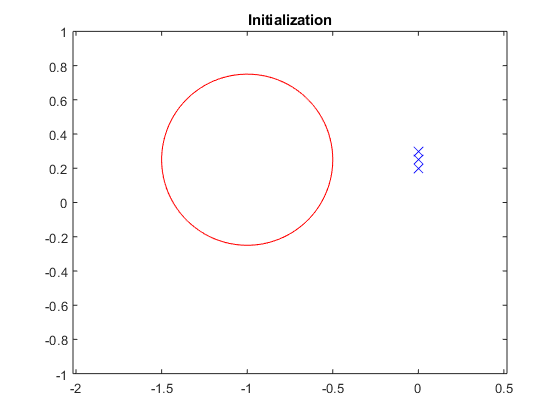
\includegraphics[scale = 0.3]{x0_1_start.png}
				&
				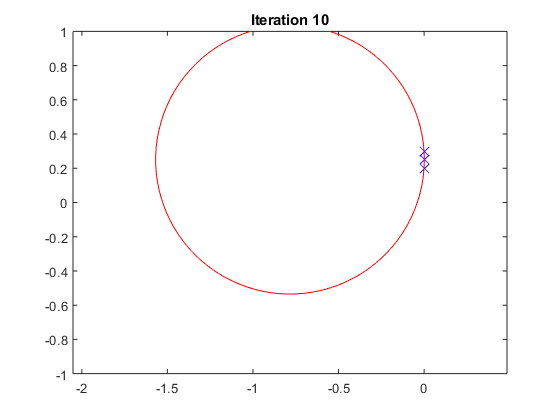
\includegraphics[scale = 0.3]{x0_1_end.png}
				&
				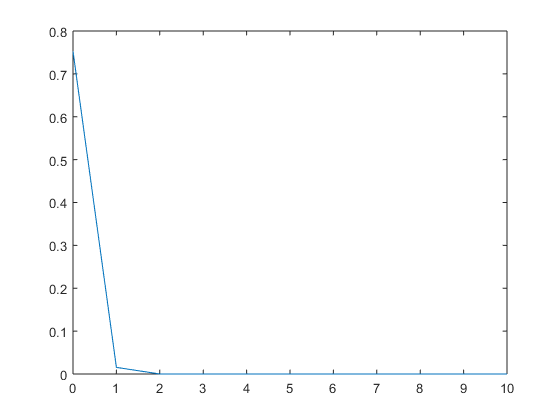
\includegraphics[scale = 0.3]{x0_1_error.png} \\
				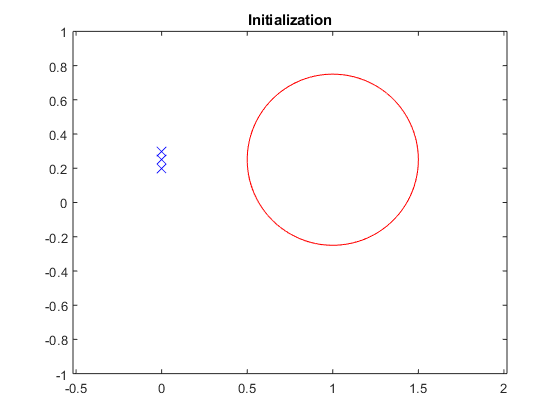
\includegraphics[scale = 0.3]{x0_2_start.png}
				&
				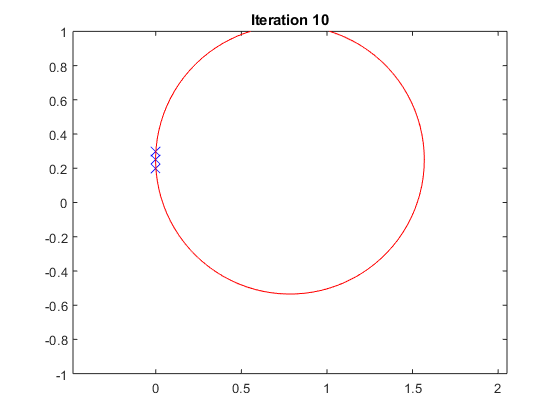
\includegraphics[scale = 0.3]{x0_2_end.png}
				&
				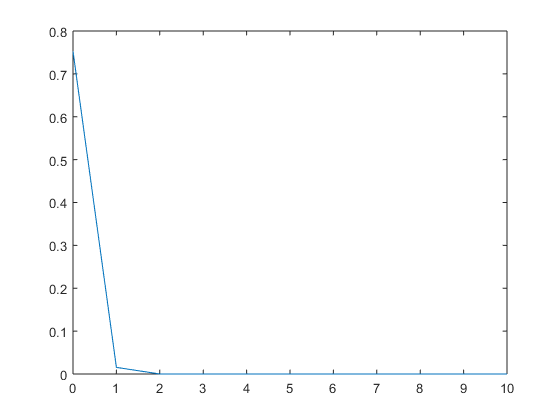
\includegraphics[scale = 0.3]{x0_2_error.png} \\

			\hline
		\end{tabular}
	\end{center}
\end{enumerate}

\end{document}